\capitulo{3}{Conceptos teóricos}

En este apartado se van a explicar los distintos conceptos teóricos necesarios para comprender correctamente el proyecto.

\section{Vídeo}
El vídeo es un tipo de datos compuesto por un conjunto de imágenes, y en algunos casos, una señal de audio sincronizada con ellas. Existen diversos formatos para vídeo que dependen de la codificación de los datos que utiliza, pero los más comunes son \textit{mp4}, \textit{avi}, \textit{webm}\ldots Aparte de la compresión de la propia codificación, el tamaño de este tipo de datos depende principalmente de dos factores: la cantidad de fotogramas por segundo y la resolución de los fotogramas.
\subsection{Fotogramas por segundo -- FPS}
Los fotogramas por segundo son una medida esencial en los vídeos que determina la cantidad de imágenes que hay por cada segundo de vídeo. Esta medida está muy relacionada con la finalidad del vídeo, ya que no se necesitan los mismos fotogramas por segundo para una película, que suele ser 24 fps~\cite{fpscine}, que para ver un documental de deporte. Cabe destacar, que a la hora de visualizar un vídeo es importante la tasa de refresco del monitor, para que se pueda apreciar correctamente la cantidad de fotogramas por segundo del vídeo se necesita una tasa de refresco igual o superior. Esto quiere decir que si un vídeo está a 60 fps lo recomendable para ver correctamente el vídeo es que el monitor tenga al menos 60Hz de tasa de refresco.
\subsection{Calidad o resolución}
La calidad de las imágenes del vídeo es otro de los parámetros más importantes, ya que dependiendo de este valor el vídeo pesará más o menos o se verá mejor o peor. Actualmente la proporción más normal de pantalla es 16:9, las calidades más comunes para esta proporción son:
\begin{itemize}
	\item 480p $\rightarrow$ 854 x 480.
	\item 720p HD $\rightarrow$ 1280 x 720.
	\item 1080p Full HD $\rightarrow$ 1920 x 1080.
	\item 1440p QHD $\rightarrow$ 2560 x 1440.
\end{itemize}
\section{Visión por computador}
La visión por computador, también llamada visión artificial, es la parte de la ciencia de la computación orientada a la recogida y al tratamiento de imágenes y vídeos~\cite{wiki:visionartifical,cnn} para la obtención de información inherente a estos tipos de datos.

Por la tipología de los datos con los que se trabaja en la visión por computador, el procesamiento de éstos es muy costoso. El elevado coste computacional es causado en gran parte por la calidad de las imágenes y en el caso de los vídeos, además de la calidad de la imagen, por la cantidad de fotogramas por segundo con el que ha sido grabado.

\subsection{Estimación de la posición o postura}
Una de las principales funciones que tiene la visión artificial es la detección de movimiento, la cual consiste en primero detectar la posición de cada una de las partes del cuerpo (depende del propio algoritmo la división que se quiera realizar sobre el cuerpo) para posteriormente realizar un seguimiento de estos elementos. Un ejemplo de este tipo de funcionalidad se puede ver en la figura~\ref{fig:keypoint}.

\subsection{Segmentación}
Es otra de las funciones más usadas de la visión por computador, en ella se busca analizar la imagen para poder detectar y delimitar el espacio de los distintos objetos, personas o animales que hay en la imagen, como se puede ver en el ejemplo de la figura~\ref{fig:segmentation}. Este espacio delimitado se obtiene de dos formas principalmente:
\begin{itemize}
	\item Figura exacta, se delimita la silueta del objeto, persona o animal detectado con un conjunto de puntos que representan la silueta de éste.
	\item Forma geométrica, es el tipo más usado debido a que requiere menor capacidad de cómputo. La forma más utilizada es el rectángulo, pero se podrían usar otro tipo de formas para delimitar y segmentar el objeto, persona o animal detectado.
\end{itemize}

\begin{figure}[ht]
	\begin{subfigure}{.5\textwidth}
		\centering
		% include first image
		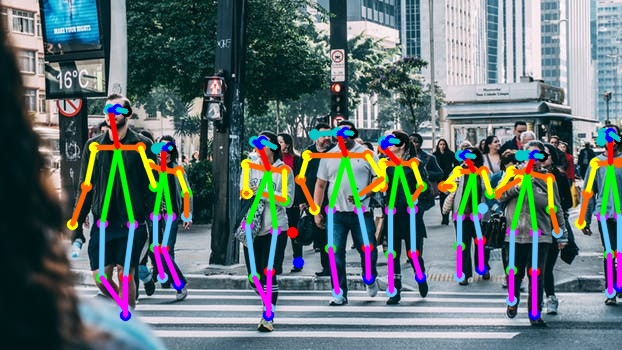
\includegraphics[width=.8\linewidth,height=4cm]{keypoint}  
		\caption{Ejemplo estimación de la postura.}
		\label{fig:keypoint}
	\end{subfigure}
	\begin{subfigure}{.5\textwidth}
		\centering
		% include second image
		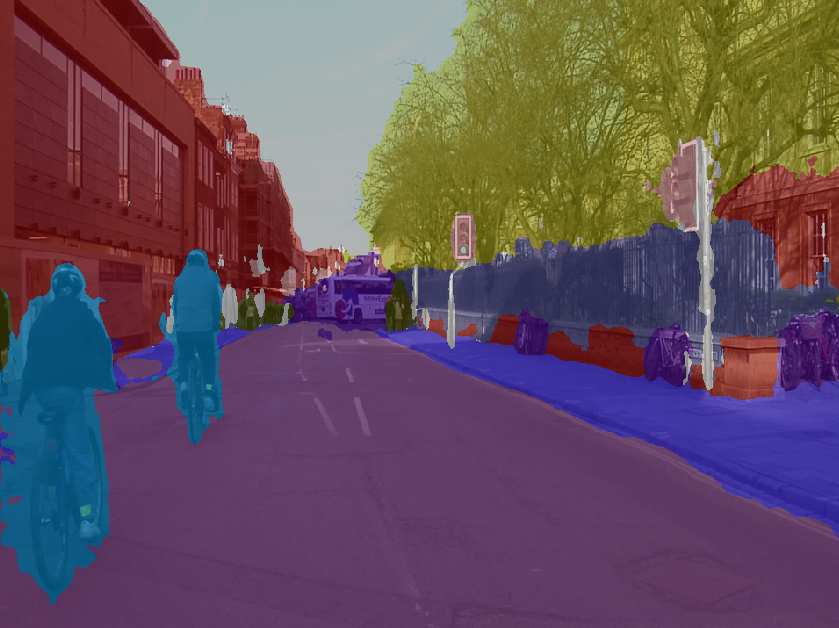
\includegraphics[height=4cm]{segmentacion}  
		\caption{Ejemplo segmentación.}
		\label{fig:segmentation}
	\end{subfigure}
	\caption{Ejemplos tipos de utilidades de la visión por computador.}
	\label{fig:vc}
\end{figure}

\section{Redes neuronales}
Son modelos basados en la analogía con la corteza cerebral de los mamíferos, aunque no están cerca, al menos de momento, de ser tan complejos como el cerebro biológico. El funcionamiento de estos modelos es relativamente sencillo, ya que <<solo>> son un conjunto de unidades básicas (también llamadas neuronas), que reciben una entrada y devuelven una salida. Donde realmente reside su complejidad, al igual que en el cerebro humano, es en las conexiones de estas unidades básicas para formar un modelo complejo capaz de realizar multitud de tareas~\cite{cnn}.

Estas unidades interactúan con los datos que les llegan mediante una función de activación que puede excitar a esta unidad o neurona y así pasar la información modificada a sus conexiones. Además, las distintas conexiones entre las unidades tienen un peso definido, que expresa la fuerza del enlace. Este peso se modifica a lo largo del entrenamiento de la red para poder obtener mejores resultados.

Según como se propague la información por la red, estas pueden dividirse en dos tipos:
\begin{itemize}
	\item \textbf{\textit{Feed-forward networks}:} redes neuronales donde la información solo avanza por ésta hacia delante, no existe ningún tipo de bucle entre las conexiones de las unidades que haga pasar la información dos o más veces por una de éstas. En este tipo de redes neuronales se encuentran el perceptrón multicapa y las redes neuronales convolucionales.
	\item \textbf{\textit{Feed-back networks}:} redes neuronales que sí admiten bucles entre sus conexiones, lo que les permite tener capacidad de memorización. Algún ejemplos de este tipo de redes son las redes neuronales recurrentes o las \textit{Long-Short Term Memory}~\cite{lstm}.
\end{itemize}
\subsection{Redes neuronales convolucionales}
Las redes neuronales convolucionales o CNNs~\cite{cnn}, de sus siglas en inglés Convolutional Neural Network, son de los tipos de redes más usados en la actualidad, sobre todo cuando se trabaja con datos de alta dimensionalidad, principalmente imágenes y vídeos. Las redes neuronales convolucionales tienen dos fases (figura~\ref{fig:cnn}):
\begin{enumerate}
	\item Fase de extracción de características.
	\item Fase de clasificación, puede realizarse con un perceptrón multicapa por ejemplo.
\end{enumerate}

\begin{figure}[h]
	\centering
	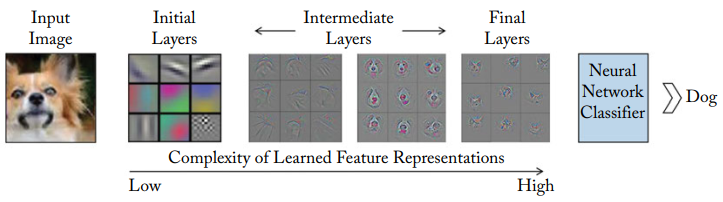
\includegraphics[width=1\textwidth]{cnn}
	\caption[Organización de una red neuronal convolucional.]{Organización de una red neuronal convolucional~\cite{cnn}.}
	\label{fig:cnn}
\end{figure}

Cada fase está relacionada con un paradigma de aprendizaje distinto, ya que en la extracción de características a partir de filtros se realiza de forma no supervisada, mientras que en la fase de clasificación se realiza un aprendizaje supervisado a partir de los datos obtenidos en la fase de extracción de características.


Aun así, el primer paso que siempre se ha de llevar a cabo antes de entrar en las distintas capas es realizar un preprocesado de la imagen. Éste puede realizarse mediante:
\begin{itemize}
	\item Substracción de la media, para a partir de ésta poder centrar los datos. Para cada dato de entrenamiento $x$ de un conjunto $N$ tal que $x \epsilon \mathbb{R}^{h*w*c}$, donde $h$ es el alto de la imagen, $w$ es el ancho y $c$ es color (normalmente 3 dimensiones, RGB), se puede definir la extracción de la media con la siguiente fórmula:
	\begin{equation}
	x'=x-\widehat{x}, \widehat{x}=1/N\sum_{i=1}^{N}x_i
	\end{equation}
	\item Normalización. Con la fórmula:
	\begin{equation}
	x''=\frac{x'}{\sqrt{\frac{\sum_{i=1}^{N}(x_i-\widehat{x})^2}{N-1}}}
	\end{equation}
	\item Blanqueo con PCA para reducir las correlaciones entre las diferentes dimensiones de los datos a partir de un normalización independiente para cada una de ellas.
	\item \textit{Local Contrast Normalization}, tipo de normalización que permite resaltar los valores más elevados.
\end{itemize}

Los tipos de preprocesados que se suelen realizar son la substracción de la media y la normalización, que a la vez son los métodos más sencillos.

\subsubsection{Tipos de capas en una red neuronal convolucional}
A continuación se exponen los tipos de capas más comunes en una red neuronal convolucional.

\textbf{Capas convolucionales}

Como ya se ha comentado, la funcionalidad de estas capas es la extracción de características a partir de filtros, pero ¿qué es un filtro? Un filtro es una malla con valores discretos, normalmente cuadrada, que representan pesos que se modifican en la fase de entrenamiento de la red. Es con cada uno de estos filtros con los que se recorren los datos para obtener como resultado un resumen de los datos de entrada. Como se ve en la figura~\ref{fig:filtro}, el resumen se calcula aplicando el filtro a los datos multiplicando los valores de los datos por su posición en el filtro y luego sumando los valores.

Al aplicar el filtro hay que tener en cuenta el \textit{stride}, que es el movimiento que hace el filtro en cada paso, en la imagen se puede ver como este valor es de 1 por lo que la imagen avanza horizontal y verticalmente de uno en uno. Valores más altos de \textit{stride} producen resúmenes más comprimidos pero puede que menos precisos, lo que se suele llamar un submuestreo de los datos.

\begin{figure}[h]
	\centering
	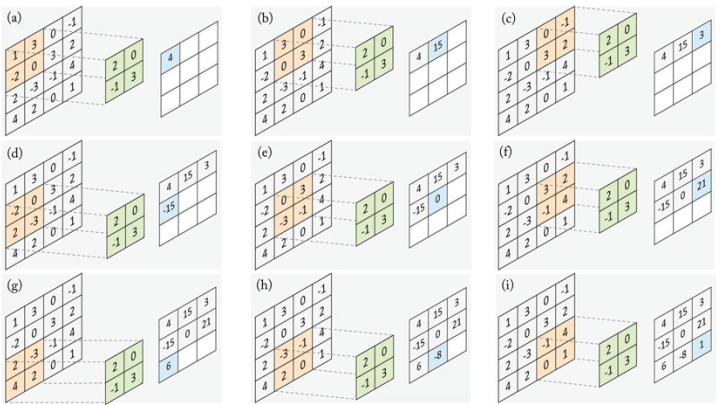
\includegraphics[width=1\textwidth]{filtro}
	\caption[Ejemplo aplicación de un filtro con \textit{stride} 1.]{Ejemplo aplicación de un filtro con \textit{stride} 1~\cite{cnn}.}
	\label{fig:filtro}
\end{figure}

Para calcular el tamaño de los datos una vez pasado un filtro se puede usar la siguiente fórmula, donde $h$ es \textit{height} (alto), $w$ es \textit{width} (ancho), $s$ es el \textit{stride} y $f$ es el tamaño del filtro:
\begin{equation}
h'=\left \lfloor \frac{h-f+s}{s} \right \rfloor; w'= \left \lfloor \frac{w-f+s}{s} \right \rfloor
\end{equation}

Siendo $\left \lfloor x  \right \rfloor$ la función de parte entera o \textit{floor operation} de $x$. Si se aplica esta fórmula a los datos de la imagen~\ref{fig:filtro}:

\begin{equation}
h'=\left \lfloor \frac{4-2+1}{1} \right \rfloor = 3; w'= \left \lfloor \frac{4-2+1}{1} \right \rfloor=3
\end{equation}

Con este tipo de capas existe un problema, ya que hay muchas situaciones que necesitan que se conserve el tamaño de los datos, como por ejemplo en una segmentación, pero si se utiliza este tipo de capas aunque se use el valor mínimo, \textit{stride} 1, se siguen perdiendo datos suavizando sobre todo los bordes. Es por ello que surgió el concepto \textit{zero-padding} que permite mantener el tamaño original de los datos.

El \textit{zero-padding} consiste añadir a los datos de entrada bordes con valores 0 para que cuando se pase el filtro el tamaño de los datos se intente mantener constante. Con el uso del \textit{zero-padding} la fórmula se modifica usando $p$ como el número de aumentos con valores a 0 en cada dimensión~\cite{zeropadding}:
\begin{equation}
h'=\left \lfloor \frac{h-f+s+p}{s} \right \rfloor; w'= \left \lfloor \frac{w-f+s+p}{s} \right \rfloor
\end{equation}

El uso de \textit{padding} se puede dividir en 3 categorías:
\begin{itemize}
	\item \textit{Valid Convolution}: es el caso más sencillo, el filtro siempre se mantiene en posiciones válidas. Las dimensiones finales se reducen tanto en el alto ($h$) como en ancho ($w$) en el tamaño del filtro ($f$) menos 1.
	\item \textit{Same Convolution}: en este caso los datos de entrada y de salida de la capa tienen el mismo tamaño, para conseguirlo se ha de realizar \textit{zero-padding} correctamente, ya que no se puede dar en todos los casos.
	\item \textit{Full Convolution}: en este caso se utiliza el mayor \textit{padding} posible, que se consigue cuando solo un elemento de los datos de entrada está involucrado en todas las operaciones con el filtro.
\end{itemize}

Como se puede ver, el \textit{stride} y sobre todo el tamaño del filtro a aplicar es muy importante en este tipo de capas, es por ello que definir un buen valor para estos puede ser esencial en el desarrollo del modelo. Por esta razón existe la función de \textit{Receptive Field} que permite descubrir el valor para el tamaño de los filtros (todos los filtros de todas las capas del mismo tamaño) más efectivo. La fórmula del \textit{Effective Receptive Field} para la capa $N$ de las $N$ capas convolucionales es:

\begin{equation}
RF_{eff}^n = f + n*(f-1)
\end{equation}

Pero, como se ha visto, los filtros no suelen tener el mismo tamaño ni el mismo \textit{stride}, es por ello que la función de \textit{Receptive Field} para el tamaño de más de un filtro es:

\begin{equation}
RF_{eff}^n = RF_{eff}^{n-1} + ((f_n -1)* \prod_{i=1}^{n-1}s_i)
\end{equation}

Donde $f_n$ es el tamaño del filtro de la capa $n$, $s_i$ es el valor de \textit{stride} para la capa $i$, y $RF_{eff}^{n-1}$ representa el \textit{effective receptive field} de la capa anterior.

Como ya se ha comentado, uno de los principales problemas de las capas convolucionales son los valores de los bordes, ya que al aparecer menos en las operaciones de los bordes se ven menos representados en las salidas de las capas. Es por ello que se propuso una modificación de las capas convolucionales llamada \textit{Dilated Convolution}, la cual tiene una dilatación ($d$) siendo esta la distancia entre los valores del filtro a tener en cuenta. Como se puede ver en la figura~\ref{fig:dilated}, donde se obtiene un filtro de tamaño 3 y con una dilatación de 2, los valores de los bordes tienen un mayor peso en la salida de la capa.

\begin{figure}[h]
	\centering
	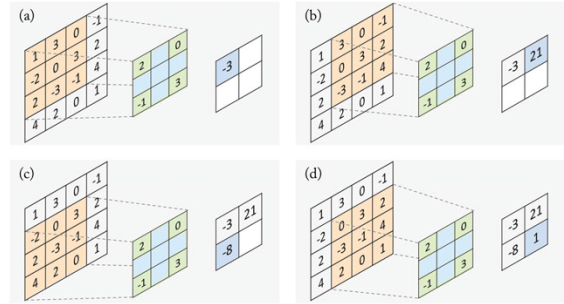
\includegraphics[width=1\textwidth]{dilated}
	\caption[\textit{Dilated Convolution} con dilatación a 2.]{\textit{Dilated Convolution} con dilatación a 2~\cite{cnn}.}
	\label{fig:dilated}
\end{figure}

Al haber añadido un nuevo parámetro, el tamaño de la salida viene dado por las siguiente fórmulas:

\begin{equation}
\begin{split}
h'=\frac{h-f-(d-1)*(f-1)+s+2p}{s}\\w'=\frac{w-f-(d-1)*(f-1)+s+2p}{s}
\end{split}
\end{equation}

\textbf{Capas de agrupación}

Tipo de capa en la cual se realiza una agrupación por un número fijado de datos. Esta agrupación se puede realizar de diversas formas, como puede ser la media, el mínimo o el máximo, entre otros. Como en las capas convolucionales, se ha de pasar el valor del \textit{stride} para indicar cómo va a ser el movimiento del segmento de agrupación. Además, se le ha de pasar el tamaño del segmento de agrupación, algo parecido a lo que pasaba con el tamaño del filtro, pero en este caso no hay valores en el filtro, simplemente se agrupan siguiendo una función los datos del segmento. Un ejemplo se puede ver en la figura~\ref{fig:agrupacion}, donde se puede observar como los valores se van agrupando acorde con el valor máximo del segmento o bloque comprobado. Los tamaños de las salida de los datos tras pasar por una capa se pueden calcular con las siguiente fórmulas, donde $f$ pasa a ser el tamaño del segmento o bloque:

\begin{equation}
h'=\left \lfloor \frac{h-f+s}{s} \right \rfloor;w'=\left \lfloor \frac{w-f+s}{s} \right \rfloor
\end{equation}

\begin{figure}[h]
	\centering
	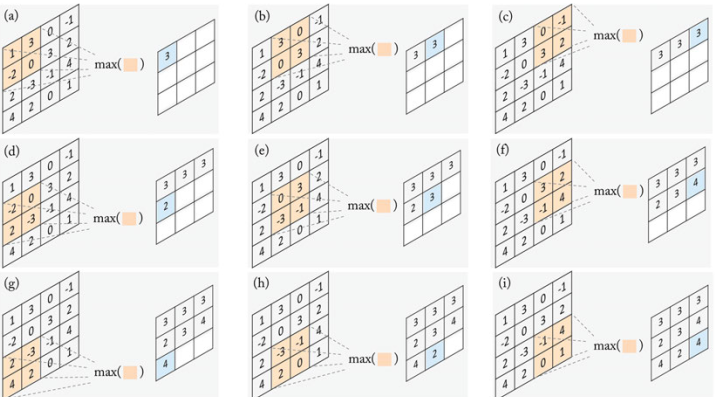
\includegraphics[width=1\textwidth]{agrupacion}
	\caption[Ejemplo de capa de agrupación de tamaño 2.]{Ejemplo de capa de agrupación de tamaño 2~\cite{cnn}.}
	\label{fig:agrupacion}
\end{figure}

Este tipo de capas son muy útiles para compactar la información y para detectar cambios en los datos, como puede ser el movimiento o la posición en una imagen.

\textbf{Capas totalmente conectadas}

Tipo de capa en la cual todas sus unidades están conectadas con todas las unidades de la capa anterior. En este tipo de capas se realiza una operación parecida a las capas convolucionales, salvo que en este caso se realiza con una tamaño de filtro de 1, es decir, se realiza la operación dato a dato. 

\textbf{Capas de no linealidad}

Capas en las cuales la función de activación de cada unidad toma como valor de entrada un número y da como salida un valor en un rango corto, como puede ser [0,1] o [-1,1]. Este tipo de capas suele ir después de las capas <<pesadas>> como las capas convolucionales o de las capas totalmente conectadas. Este tipo de capa es muy importantes utilizarlas después de las capas <<pesadas>> debido a que permite mapear espacios no lineales. Algunas de las funciones de activación de esta capa más comunes se pueden ver en la figura~\ref{fig:funac}.

\begin{figure}[h]
	\centering
	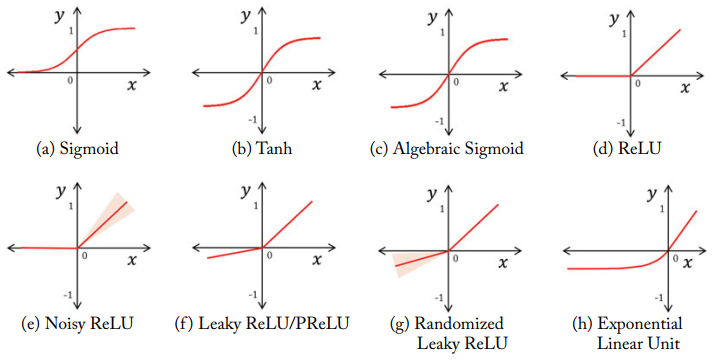
\includegraphics[width=1\textwidth]{funac}
	\caption[Funciones de activación más comunes en capas de no linealidad.]{Funciones de activación más comunes en capas de no linealidad~\cite{cnn}.}
	\label{fig:funac}
\end{figure}
\subsection{ResNet}
ResNet o \textit{Residual Network} es un tipo de arquitectura de redes neuronales convolucionales creada por Microsoft~\cite{resnet}. Este tipo de CNN se caracterizan por saltarse las conexiones de identidad en los bloques residuales, para así obtener un modelo mucho más sencillo de entrenar. En un bloque residual, los datos de entrada se duplican, pasando unos por las transformaciones y otros por las conexiones de identidad, estas conexiones, como se puede ver en la figura~\ref{fig:resnet}, sirven para saltarse las capas de transformación, pasando los datos iniciales tal cual llegan.

\begin{figure}[h]
	\centering
	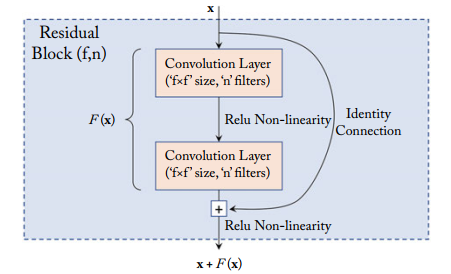
\includegraphics[width=0.5\textwidth]{resnet}
	\caption[Ejemplo bloque residual en ResNet.]{Ejemplo bloque residual en ResNet~\cite{cnn}.}
	\label{fig:resnet}
\end{figure}
\subsection{Region-Based CNN}
Las \textit{Region-Based Convolutional Neural Networks} o RCNN son un tipo de redes neuronales convolucionales orientadas al reconocimiento de objetos en imágenes. Este tipo de redes convolucionales, como se puede observar en la figura~\ref{fig:rcnn}, tiene 3 módulos~\cite{cnn}:
\begin{itemize}
	\item Módulo de extracción de propuestas a región.
	\item Módulo de extracción de características. Uso de redes neuronales convolucionales para la extracción de características de cada región propuesta.
	\item Módulo de clasificación de regiones. Se entrena un SVM (Support Vector Machine) por cada clase a predecir, después se usa para clasificar las regiones a partir de las características extraídas en el módulo anterior.
\end{itemize}
\begin{figure}[h]
	\centering
	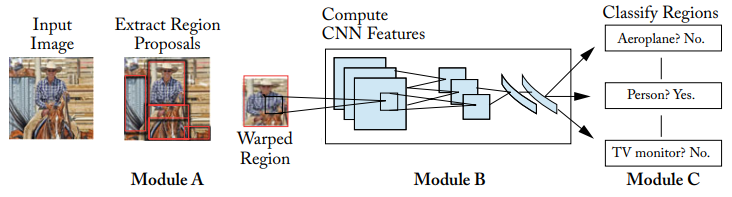
\includegraphics[width=1\textwidth]{rcnn}
	\caption[Region-Based CNN.]{Region-Based CNN~\cite{cnn}.}
	\label{fig:rcnn}
\end{figure}
\subsection{FPN}
FPN o Feature Pyramid Network es un tipo de red neuronal piramidal que se utiliza junto con las redes neuronales convolucionales para tareas relacionadas con las imágenes, tales como la detección de objetos (usándose junto una RCNN) o la segmentación. Este tipo de redes, como se puede observar en la figura~\ref{fig:fpn}, tiene dos fases~\cite{fpn}:
\begin{itemize}
	\item \textit{Bottom-up pathway}: Fase en la cual se utiliza la red neuronal convolucional para extraer características de la imagen, como por ejemplo con ResNet. Cada capa dentro de esta red neuronal convolucional es de la mitad del tamaño que la anterior (por lo que hay que tener en cuenta todos los atributos de las capas de una red neuronal ya comentados). En el ejemplo de ResNet se obtiene la salida de cada capa como el resultado de cada bloque residual.
	\item \textit{Top-down pathway and lateral connections}: En esta fase, en el primer nivel, se toma como entrada la salida de la última capa de la fase anterior, y se va bajando de nivel pasando al siguiente nivel la predicción del anterior y la salida de la capa de la red neuronal que está al mismo nivel.
\end{itemize}
\begin{figure}[h]
	\centering
	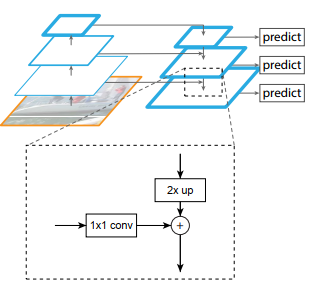
\includegraphics[width=0.5\textwidth]{fpn}
	\caption[Feature Pyramid Network.]{Feature Pyramid Network~\cite{fpn}.}
	\label{fig:fpn}
\end{figure}

\section{Puntos y vectores}
El punto es la representación mínima en una espacio, donde representa una posición exacta dentro de este espacio. Un punto dentro de un espacio se representa con tantos valores como dimensiones tiene el espacio donde se encuentra.

El vector es otro de los conceptos básicos matemáticos que se define como un segmento orientado. Un vector se representa a partir de 3 valores, su módulo o longitud del segmento, su dirección y su sentido.

Este concepto de vector, o incluso conceptos con mayor número de dimensiones como son las matrices, es muy utilizado en la programación. Uno de los tipos más conocidos de matrices multidimensionales que trabaja con solo un tipo de dato son los \textit{tensores}, matrices multidimensionales implementadas para optimizar las operaciones en la GPU (tarjeta gráfica)~\cite{tensor}. 

\subsection{Distancia entre puntos}
La distancia entre dos puntos es el espacio que los separa. Esta distancia se puede calcular de distintas formas, ya que depende mucho del espacio en el que se encuentren los puntos. Algunas de las distancias más comunes son:
\begin{itemize}
	\item \textbf{Manhattan}: distancia que se calcula como la suma de las diferencia de los valores de las distintas dimensiones de los puntos.
	\item \textbf{Euclídea}: distancia que se calcula como la longitud de la línea que une los dos puntos, a partir del teorema de Pitágoras.
\end{itemize}
